\documentclass[journal]{IEEEtran}

\usepackage[T1]{fontenc}
\usepackage{cite}
\usepackage{amsmath,amssymb,amsfonts,amsthm}
\usepackage{graphicx}
\usepackage{booktabs}
\usepackage{multirow}
\usepackage{array}
\usepackage{microtype}
\usepackage{url}
\usepackage[hidelinks]{hyperref}
\usepackage{tikz}
\usetikzlibrary{arrows.meta,positioning,calc}

\newtheorem{proposition}{Proposition}

\begin{document}

\title{Freshness- and Stall-Aware Multipath QUIC Scheduling for Deadline-Constrained IoT Traffic: Real-Stack Evaluation}

\author{Weicheng~Tong%
\thanks{W.~Tong is with Shandong Agricultural Engineering University, Jinan, Shandong, China. Generative AI tools assisted with language editing, experiment-script drafting, and \LaTeX{} typesetting; the author conceived the design, implemented and verified all C/XQUIC schedulers, proofs, and real-stack experiments, and takes full responsibility for all claims. Reproducible C/XQUIC source code, Linux \texttt{netns}/\texttt{netem} scripts, independent Oracles, and 1,596+ audited connection archives are maintained at \url{https://github.com/Sver0411/IoT-MPQUIC-Scheduler}.}}

\markboth{FAP-MPQUIC: FRESHNESS- AND STALL-AWARE MULTIPATH QUIC SCHEDULING FOR IOT TRAFFIC}%
{Tong: FAP-MPQUIC for Deadline-Constrained IoT Traffic}

\maketitle

\begin{abstract}
Industrial and cyber-physical Internet of Things (IoT) gateways increasingly aggregate dual heterogeneous links (e.g., Wi-Fi plus cellular or Sub-GHz backhaul) using Multipath QUIC (MPQUIC) to carry both sporadic, hard-deadline alarm events and overwriteable periodic state telemetry. Classical multipath schedulers---including native MinRTT, Earliest Completion First (ECF), and BLEST---optimize bulk throughput using cached round-trip times (RTT) and ignore deadline slack, overwrite freshness (Age of Information, AoI), and stale-RTT blindness on idle backup paths. Consequently, when the primary path suffers an asymmetric reversal or silent blackout, classical schedulers remain trapped on the degraded path and miss critical deadlines. We present \texttt{FAP-MPQUIC}, a lightweight C multipath scheduler built directly on Alibaba's production \texttt{XQUIC} (\texttt{XQC\_MULTIPATH\_10}) stack that pairs a freshness- and deadline-aware application queue with CWND-blocking-aware timely delivery estimation and health-gated stale-path freshness probing (using zero extra control frames). Across a held-out real-stack evaluation of 576 dual-path \texttt{XQUIC} connections (16 independent seeds $\times$ 4 dynamic Linux \texttt{netns}/\texttt{tc-netem} regimes $\times$ 9 policies, complemented by 1,020+ mechanism, failover, and calibration connections), \texttt{FAP-MPQUIC} boosts event deadline success by \textbf{+20.6 to +22.2\,pp} under high-load outage-reversal ($p_{\text{Holm}}{\le}0.0025$) and by \textbf{+21.5 to +52.1\,pp} under mid-connection blackout ($p_{\text{Holm}}{\le}0.0230$) over \texttt{FIFO+MinRTT}, \texttt{App+MinRTT}, \texttt{Fixed-MinRTT}, \texttt{ECF}, and \texttt{BLEST}, while strictly Pareto-dominating all four classical path schedulers on event delivery, state AoI ($-$168 to $-$308\,ms), and useful goodput ($+$8.9 to $+$9.8\,kbps). Under non-blackout asymmetric and double reversals---where probability-only binding (\texttt{Prob-Only}) and no-probe ablations remain caught in stale cached RTTs---health-gated probing achieves the lowest observed AoI of all 9 policies (1,927--1,940\,ms; $-$70.1\,ms vs.\ \texttt{FAP-NoProbe}, $p_{\text{Holm}}{=}0.0123$) with zero blackout credit waste. Independent mechanism analyses further quantify cross-path repair ($-$83.6\% outage-probe latency) and offline calibration boundaries transparently.
\end{abstract}

\begin{IEEEkeywords}
Age of Information (AoI), deadline-aware scheduling, Internet of Things (IoT), Multipath QUIC (MPQUIC), path probing, XQUIC.
\end{IEEEkeywords}

\section{Introduction}
\IEEEPARstart{M}{odern} edge gateways in smart agriculture, industrial monitoring, and connected robotics frequently possess dual heterogeneous wireless interfaces---such as local Wi-Fi alongside cellular LTE/5G or Sub-GHz backhaul---to protect time-critical sensing streams against single-link congestion, fading, and blackouts~\cite{deconinck2017mpquic,kahraman2024survey}. Multipath QUIC (MPQUIC), building on QUIC's stream-multiplexed UDP transport~\cite{rfc9000,rfc9002}, eliminates inter-stream head-of-line (HoL) blocking while enabling fine-grained per-stream path selection across heterogeneous interfaces~\cite{zheng2021xlink,yang2024mams}.

IoT gateway traffic, however, differs fundamentally from bulk file transfers or continuous video streams~\cite{guo2017dems,zheng2021xlink}. Gateways multiplex two conflicting record classes over a small QUIC concurrency credit window: (i) \emph{sporadic alarm events} carrying strict completion deadlines~\cite{liu1973scheduling,chen2024damps}, and (ii) \emph{periodic sensor state updates} whose utility depends on receiver freshness---quantified by Age of Information (AoI)~\cite{kaul2012realtime,yates2021age}---where newer readings supersede stale pending updates.

Evaluating real \texttt{XQUIC} connections over Linux \texttt{netns}/\texttt{tc-netem} dual paths reveals two structural failure modes in existing multipath schedulers:
\begin{enumerate}
\item \textbf{Ignoring Loss, Variance, and Deadlines:} Native \texttt{MinRTT}~\cite{rfc8684}, \texttt{ECF}~\cite{lim2017ecf}, and \texttt{BLEST}~\cite{ferlin2016blest} rank paths primarily by smoothed RTT and queue drain time without modeling deadline slack, RTT variance, or packet loss. Under sudden Path-A outages or reversals, they bind scarce QUIC stream credits onto the degraded path, collapsing event deadline delivery to 2.8--5.0\% (high-load outage) and 52.8--55.6\% (mid-run blackout).
\item \textbf{Stale-RTT Path Trap and Unchecked Probing Hazard:} Pure greedy schedulers---even loss- and probability-aware binders without probing (\texttt{Prob-Only})---pin traffic onto the initially faster Path~A, leaving Path~B's cached SRTT frozen at stale pre-reversal values ($>$1\,s old). Prior application-ACK residual adaptation proved too slow (930--960\,ms feedback lag vs.\ 25--100\,ms deadlines). Conversely, naively probing a stale path on a fixed timer wastes scarce QUIC \texttt{MAX\_STREAMS} credits whenever that alternate path is actually blacked out.
\end{enumerate}

To solve both problems cleanly inside a real C production QUIC stack, we introduce \textbf{\texttt{FAP-MPQUIC}} (Freshness- and Stall-Aware Probability MPQUIC) and make four contributions:
\begin{enumerate}
\item \textbf{Health-Gated Freshness Probing \& CWND-Aware Estimation:} \texttt{FAP-MPQUIC} augments timely delivery probability estimation with explicit \texttt{in\_flight} $>$ \texttt{cwnd} round penalties and dispatches zero-overhead freshness probes using replaceable state streams \emph{only} when a stale alternate path ($\ge$150\,ms old) is clean and idle ($\text{PTO}{=}0$, $\text{recent\_lost}{=}0$, $\text{in\_flight}{=}0$).
\item \textbf{Analytical Guarantees (Propositions~1--2):} We prove a bounded post-reversal discovery latency via transport-layer QUIC ACKs, a zero-blackout-waste invariant under Path-A blackouts, and strictly $O(K{+}|\mathcal{Q}|)$ per-submission complexity.
\item \textbf{Held-Out Real \texttt{XQUIC} Dual-Path Evaluation:} Across 576 held-out real connections (16 seeds $\times$ 4 dynamic Linux \texttt{netns}/\texttt{tc-netem} regimes $\times$ 9 policies) plus 1,020+ mechanism, failover, and calibration connections with dual-interface PCAPs and independent Oracles, we benchmark \texttt{FAP-MPQUIC} against native \texttt{MinRTT}, \texttt{Fixed-MinRTT}, \texttt{ECF}, \texttt{BLEST}, probability-only binding (\texttt{Prob-Only}), and two internal ablations (\texttt{FAP-NoProbe}, \texttt{FAP-Cross}).
\item \textbf{Two-Layer Mechanistic Clarity and Honest Boundaries:} We separate (i) blackout regimes, where loss- and slack-aware probability binding dominates classical RTT schedulers, from (ii) non-blackout asymmetric and double reversals, where health-gated probing breaks the stale-RTT trap ($-$70.1\,ms vs.\ \texttt{FAP-NoProbe}, $p_{\text{Holm}}{=}0.0123$) with zero blackout credit waste, alongside transparent failover and calibration analyses.
\end{enumerate}

\section{Related Work}
\paragraph{Multipath Transport and Heuristic Schedulers}
Multipath TCP (RFC~8684~\cite{rfc8684}) and Multipath QUIC~\cite{deconinck2017mpquic} enable concurrent transmission over heterogeneous links using QUIC's loss detection and CUBIC congestion control~\cite{rfc9000,rfc9002,ha2008cubic}. To mitigate HoL blocking across asymmetric paths, Ferlin et al.~\cite{ferlin2016blest} proposed \texttt{BLEST} to avoid slow paths that block the fast path's send window; Lim et al.~\cite{lim2017ecf} introduced \texttt{ECF} to wait for the fast path when it completes earlier; Guo et al.~\cite{guo2017dems} developed \texttt{DEMS} for synchronized chunk completion; and Zeng et al.~\cite{zeng2022optimizing} optimized MPQUIC scheduling over heterogeneous paths to curb lowest-RTT-first inefficiencies. Production systems such as Alibaba's \texttt{XLINK}~\cite{zheng2021xlink} demonstrate MPQUIC QoE gains in large-scale video delivery. However, these schedulers optimize bulk completion time rather than mixed IoT deadlines and overwriteable state freshness.

\paragraph{Learning-Based and Deadline-Aware MPQUIC}
To cope with dynamic wireless paths, \texttt{Peekaboo}~\cite{wu2020peekaboo} applies multi-armed bandits in MPQUIC, while recent works introduce mobility-aware scheduling (\texttt{MAMS}~\cite{yang2024mams}), contextual bandits (\cite{yang2024qos}), meta-RL for live video (\texttt{Meta-DAMS}~\cite{sepahi2024metadams}), cost-aware VoD multipath splitting for 5G ATSSS~\cite{amend2024cost}, and deadline-aware packet scheduling for real-time mobile video/XR (\texttt{DaMPS}~\cite{chen2024damps}). Crucially, these recent deadline-aware and RL/MAB controllers target continuous video-frame or chunk streaming rather than IoT overwriteable AoI semantics plus sporadic hard-deadline alarms, and incur online exploration variance that complicates deterministic per-stream Oracle auditing inside a compact C transport callback. Calibration under distribution shift~\cite{guo2017calibration,ovadia2019uncertainty} further warns that uncalibrated probability predictors can misrank paths after sudden link shifts---a phenomenon we verify directly on \texttt{XQUIC} traces.

\paragraph{Age of Information and IoT Scheduling}
Since Kaul et al.~\cite{kaul2012realtime}, AoI optimization over unreliable IoT networks has expanded across stochastic arrivals~\cite{yates2021age,kadota2021minimizing,kahraman2024survey}, semantic staleness~\cite{maatouk2020aoii}, nonlinear Whittle indices~\cite{tripathi2024whittle}, soft AoI deadlines~\cite{li2025soft}, heterogeneous access~\cite{wu2024paoi}, edge offloading~\cite{jiang2023aoi}, and Sub-GHz LPWAN scheduling~\cite{garridohidalgo2021lorawan,lima2021adaptive}. Most AoI schedulers assume single-path slotted models rather than real encrypted MPQUIC stacks with CUBIC pacing, \texttt{MAX\_STREAMS} credit limits, and PTO recovery. Our work bridges real MPQUIC transport engineering with AoI- and deadline-aware IoT scheduling.

\section{System Architecture and FAP-MPQUIC Design}

Fig.~\ref{fig:arch} illustrates our end-to-end dual-path \texttt{XQUIC} architecture. A gateway client and receiver communicate over one MPQUIC connection (\texttt{XQC\_MULTIPATH\_10}, CUBIC + pacing, initial unidirectional stream credit $C{=}4$, active window $W{=}8$) spanning two isolated Linux \texttt{veth} interfaces (\texttt{Path~A} and \texttt{Path~B}) controlled by timed \texttt{tc-netem} schedules.

\begin{figure*}[t]
\centering
\resizebox{0.97\textwidth}{!}{%
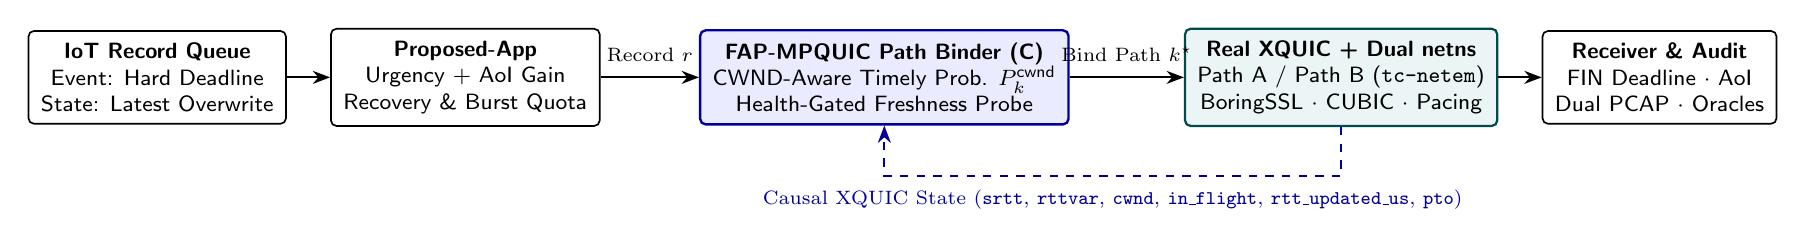
\begin{tikzpicture}[
    font=\sffamily\footnotesize,
    box/.style={draw, rounded corners=2pt, align=center, minimum height=10mm, inner sep=4.5pt, fill=white, line width=0.6pt},
    ctrl/.style={box, fill=blue!8, draw=blue!60!black, line width=0.85pt},
    hw/.style={box, fill=teal!8, draw=teal!60!black, line width=0.8pt},
    arr/.style={-{Stealth[length=2.2mm]}, line width=0.75pt},
    dasharr/.style={-{Stealth[length=2.2mm]}, dashed, line width=0.75pt, draw=blue!60!black}
]
\node[box] (q) {\textbf{IoT Record Queue}\\Event: Hard Deadline\\State: Latest Overwrite};
\node[box, right=0.55cm of q] (app) {\textbf{Proposed-App}\\Urgency + AoI Gain\\Recovery \& Burst Quota};
\node[ctrl, right=1.25cm of app] (fap) {\textbf{FAP-MPQUIC Path Binder (C)}\\CWND-Aware Timely Prob. $P_k^{\text{cwnd}}$\\Health-Gated Freshness Probe};
\node[hw, right=1.45cm of fap] (xqc) {\textbf{Real XQUIC + Dual netns}\\Path A / Path B (\texttt{tc-netem})\\BoringSSL $\cdot$ CUBIC $\cdot$ Pacing};
\node[box, right=0.55cm of xqc] (rx) {\textbf{Receiver \& Audit}\\FIN Deadline $\cdot$ AoI\\Dual PCAP $\cdot$ Oracles};

\draw[arr] (q.east) -- (app.west);
\draw[arr] (app.east) -- node[above=2pt, font=\scriptsize]{Record $r$} (fap.west);
\draw[arr] (fap.east) -- node[above=2pt, font=\scriptsize]{Bind Path $k^\star$} (xqc.west);
\draw[arr] (xqc.east) -- (rx.west);
\draw[dasharr] (xqc.south) -- ++(0,-0.62) -| node[pos=0.25, below=1.5pt, font=\scriptsize, text=blue!60!black]{Causal XQUIC State (\texttt{srtt}, \texttt{rttvar}, \texttt{cwnd}, \texttt{in\_flight}, \texttt{rtt\_updated\_us}, \texttt{pto})} (fap.south);
\end{tikzpicture}%
}
\caption{IoT-MPQUIC-Scheduler end-to-end architecture on production C \texttt{XQUIC}. \texttt{Proposed-App} selects the next record using overwrite state freshness and deadline urgency; \texttt{FAP-MPQUIC} binds each new unidirectional QUIC stream to Path~A or Path~B using strictly causal transport telemetry from \texttt{xqc\_send\_ctl\_t} and health-gated stale-path probing. All runs capture dual-interface PCAPs for independent Oracle auditing.}
\label{fig:arch}
\end{figure*}

\subsection{Application-Layer Queue and Freshness Scoring}
Each record $r$ is transmitted on a dedicated unidirectional QUIC stream with wire size $B = 52 + \text{payload\_len}$. For a decision at elapsed time $t$, an event's remaining deadline budget is $s = d_r - t$, while a state record's effective freshness budget is $s = \min(d_r,\, g_r + M_r) - t$ (generation time $g_r$, max age $M_r$). \texttt{Proposed-App} replaces older pending state records per sensor, discards obsolete records superseded by receiver ACKs, and partitions candidates into \texttt{event}, \texttt{normal state}, and \texttt{recovery state} ($s \le 0$). With $\operatorname{sat}(x) = x/(1+x)$ and $H = 100$\,ms, normal/event records score
\begin{equation}
\begin{aligned}
U_{\text{app}}(r, t) &= \operatorname{sat}(p_r) + 2\operatorname{sat}(\sigma_r) + G_r \\
&\quad + \operatorname{sat}\!\left(\frac{w_r}{H}\right) + \frac{H}{H + \max(0, s)},
\end{aligned}
\label{eq:app}
\end{equation}
where $G_r$ is saturated potential AoI improvement from the latest receiver ACK ($0$ for events), $w_r$ is queue wait, and bounded quotas (event burst limit $3$, recovery cadence $K{=}2$) prevent state starvation.

\subsection{FAP-MPQUIC: CWND-Aware Estimation and Health-Gated Probing}
At stream creation, the path sampler queries each active, unfrozen \texttt{XQUIC} path $k \in \{1,\dots,K\}$ for its real-time \texttt{xqc\_send\_ctl\_t} state: smoothed RTT $R_k$, RTT variance $V_k = \max(\text{rttvar}_k, 1\,\text{ms})$, estimated bandwidth $v_k$, scheduled bytes $q_k$, in-flight bytes $f_k$, congestion window $W_k$, recent packet counts $(n_k, m_k)$, PTO count $\text{pto}_k$, current monotonic clock $t_s$, and last transport RTT update timestamp $t_{\text{rtt},k}$.

\paragraph{1) CWND-Blocking-Aware Delivery Probability}
Let $Q_k = q_k + f_k + B$ be total offered bytes and $L_k = \min\!\big(0.95,\; (m_k + 1)/(n_k + 20)\big)$ be smoothed per-packet loss. Whereas the probability-only ablation (\texttt{Prob-Only}) ignores congestion window saturation, \texttt{FAP-MPQUIC} adds a linear RTT blocking round penalty whenever actual in-flight bytes already exceed $W_k$:
\begin{align}
\Delta^{\text{cwnd}}_k &= \begin{cases} R_k\,\dfrac{f_k - W_k}{\max(W_k, 1200)}, & W_k{>}0,\; f_k{>}W_k, \\ 0, & \text{otherwise}, \end{cases} \label{eq:cwnd}\\
T^{\text{cwnd}}_k &= R_k\big(0.5 + 2\,\mathbb{I}[\text{pto}_k{>}0]\big) + \frac{Q_k \cdot 10^6}{\max(v_k, 15000)} + \Delta^{\text{cwnd}}_k, \label{eq:time}\\
P^{\text{cwnd}}_k &= \mathbb{I}[s{>}0]\,\operatorname{clip}_{[0,1]}\!\left(\frac{s{-}T^{\text{cwnd}}_k{+}V_k}{2V_k}\right)(1{-}L_k)^{\lceil B/1200\rceil}. \label{eq:prob}
\end{align}
Conditioning Eq.~(\ref{eq:cwnd}) on $f_k > W_k$ rather than $Q_k > W_k$ avoids falsely penalizing a clean slow-start backup path ($W_k \approx 10$\,MSS, $f_k{=}0$) during a sudden primary blackout. Let $i^\star = \arg\max_k (P^{\text{cwnd}}_k, -T^{\text{cwnd}}_k)$ denote the greedy primary choice.

\paragraph{2) Health-Gated Stale-Path Freshness Probing}
Let $\Delta_{\text{stale},k} = \max(0, t_s - t_{\text{rtt},k})$ be path $k$'s RTT staleness and $\Delta_{\text{probe},k} = t_s - t_{\text{last\_probe},k}$ be elapsed time since our last dispatch on path $k$, with freshness horizon $\tau_{\text{stale}} = 150$\,ms. Define path $j \ne i^\star$ as \emph{probe-eligible} if and only if:
\begin{equation}
\begin{aligned}
\mathcal{E}(j) \iff{} & (\text{pto}_j{=}0) \wedge (m_j{=}0) \wedge (f_j{=}0) \\
                      & \wedge (\Delta_{\text{stale},j} \ge \tau_{\text{stale}}) \wedge (\Delta_{\text{probe},j} \ge \tau_{\text{stale}}).
\end{aligned}
\label{eq:probe_gate}
\end{equation}
\texttt{FAP-MPQUIC} dispatches record $r$ onto the stalest path $j \in \mathcal{E}$ (zero extra control packets) if and only if \emph{either} (a) $r$ is a replaceable \texttt{state} record (zero deadline risk to urgent events), \emph{or} (b) $r$ is an \texttt{event} whose primary path $i^\star$ is stressed ($\text{pto}_{i^\star}{>}0$, $W_{i^\star}{>}0 \wedge Q_{i^\star}{>}W_{i^\star}$, or $s{>}0 \wedge P^{\text{cwnd}}_{i^\star}{<}0.25$). Otherwise it binds $r$ to $i^\star$. Notice the critical safety gate $f_j{=}0 \wedge m_j{=}0 \wedge \text{pto}_j{=}0$: any path with unacknowledged in-flight bytes is already being probed---and a blacked-out path keeps $f_j{>}0$ until PTO/loss triggers---preventing repeated probes from ever burning scarce \texttt{MAX\_STREAMS} credits on a dead path. We isolate three ablations: \texttt{Prob-Only} (probability binding without Eq.~(\ref{eq:cwnd}) or Eq.~(\ref{eq:probe_gate})), \texttt{FAP-NoProbe} (Eqs.~(\ref{eq:cwnd})--(\ref{eq:prob}) without Eq.~(\ref{eq:probe_gate})), and \texttt{FAP-Cross} (adding cross-path PTO/budget repair on retransmissions).

\subsection{Analytical Properties of FAP-MPQUIC}
\begin{proposition}[Bounded Reversal Discovery and Zero-Blackout-Waste Invariant]
\label{prop:fap}
Consider a two-path MPQUIC connection where state arrivals occur with inter-arrival period $\le \delta_s$ and a reversal improves idle Path~$B$ to true RTT $R_B^{\text{new}}$ at time $t_0$:
\begin{enumerate}
\item[(i)] \emph{Bounded Discovery Time:} If Path~$B$ was idle and clean before $t_0$ ($f_B{=}m_B{=}\text{pto}_B{=}0$), \texttt{FAP-MPQUIC} dispatches a state stream onto Path~$B$ no later than $t_0 + \tau_{\text{stale}} + \delta_s$, refreshing XQUIC's transport SRTT $R_B$ via a single QUIC ACK within total latency $\le \tau_{\text{stale}} + \delta_s + R_B^{\text{new}}$---independent of application-ACK queueing delay.
\item[(ii)] \emph{Zero-Blackout-Waste Invariant:} Conversely, if Path~$A$ enters a 100\% packet blackout at $t_b$ while carrying $\ge 1$ in-flight packet ($f_A > 0$), then for every subsequent slot until loss/PTO recovery, $\mathcal{E}(A) = \text{false}$ in Eq.~(\ref{eq:probe_gate}); hence \texttt{FAP-MPQUIC} dispatches \emph{zero} probe streams onto the blacked-out path, preserving at least $C{-}1$ stream credits for the healthy path.
\end{enumerate}
\end{proposition}
\begin{IEEEproof}
For (i), once $t \ge t_0 + \tau_{\text{stale}}$ (or immediately at $t_0$ if $\Delta_{\text{stale},B} \ge \tau_{\text{stale}}$ already held), $\Delta_{\text{stale},B} \ge \tau_{\text{stale}}$ and $\Delta_{\text{probe},B} \ge \tau_{\text{stale}}$ hold concurrently with $f_B{=}m_B{=}\text{pto}_B{=}0$. The next state submission (arriving within $\le \delta_s$) satisfies Eq.~(\ref{eq:probe_gate}), binds to Path~$B$, and elicits a transport-layer QUIC ACK in $\approx R_B^{\text{new}}$, updating \texttt{ctl\_srtt} and \texttt{ctl\_iot\_rtt\_update\_us} without waiting for application ACK serialization. For (ii), while Path~$A$ drops 100\% of packets, its first unacknowledged datagram keeps $f_A > 0$ until RFC~9002 PTO/loss detection fires, upon which $\text{pto}_A > 0$ and $m_A > 0$; thus $f_A{=}0 \wedge m_A{=}0 \wedge \text{pto}_A{=}0$ is never satisfied during blackout, ensuring zero wasted probes on Path~$A$.
\end{IEEEproof}

\begin{proposition}[Per-Submission Complexity and Causal Verifiability]
\label{prop:complex}
For $K$ active paths and $|\mathcal{Q}| \le 1024$ pending records, each scheduling step runs in $O(|\mathcal{Q}| + K)$ arithmetic operations with zero heap allocation in the path binder, and every binding decision is a deterministic function of strictly causal logged snapshots.
\end{proposition}
\begin{IEEEproof}
\texttt{iot\_plan\_record} scans pending entries once ($O(|\mathcal{Q}|)$) with $O(1)$ per-entry arithmetic, and \texttt{iot\_choose\_initial\_path} performs at most two linear scans over $K{=}2$ path samples ($O(K)$) reading only monotonic XQUIC counters and \texttt{last\_probe\_us}. No dynamic allocation occurs during path selection, and every input counter is archived in the logged causal path features for offline Oracle replay.
\end{IEEEproof}

\section{Experimental Setup and Real-Stack Protocol}

All experiments execute real encrypted \texttt{XQUIC} (commit \texttt{dffd32c}) + \texttt{BoringSSL} endpoints inside isolated Linux network namespaces (\texttt{client\_ns}, \texttt{server\_ns}, Linux kernel~6.12) linked by two virtual Ethernet pairs (\texttt{iot-a}, \texttt{iot-b}) with timed \texttt{tc-netem} qdiscs and dual-interface \texttt{tcpdump} PCAP capture over a fixed 4\,s observation window. We configure the QUIC connection with an initial unidirectional stream credit limit of $C{=}4$ to model the tight concurrency budget of resource-constrained IoT gateways; operating under a compact credit window directly exposes how head-of-line credit occupation on a degraded or blacked-out path blocks subsequent deadline-critical alarms.

\paragraph{Held-Out Real-Stack Evaluation Matrix (576 Connections, 16 Seeds)}
Using 16 strictly held-out seeds (\texttt{10101--10116}, disjoint from all prior development and pilot seeds), we evaluate \textbf{9 policies}---five classical/system baselines (\texttt{FIFO+MinRTT}, \texttt{App+MinRTT}, \texttt{Fixed-MinRTT}, \texttt{ECF}~\cite{lim2017ecf}, and \texttt{BLEST}~\cite{ferlin2016blest}), probability-only binding (\texttt{Prob-Only}), two ablations (\texttt{FAP-NoProbe}, \texttt{FAP-Cross}), and \textbf{\texttt{FAP-MPQUIC}}---across four dynamic dual-path regimes (randomized arm order per seed block, identical binary workload per seed):
\begin{itemize}
\item \textbf{S1 (Outage-Reversal, high-mixed):} \texttt{A} starts at $[4\,\text{ms}, 30\,\text{Mbps}]$, suffers 100\% blackout at $120\,\text{ms}$, and recovers degraded ($[45\,\text{ms}, 6\,\text{Mbps}]$) at $850\,\text{ms}$ while \texttt{B} upgrades to $[5\,\text{ms}, 30\,\text{Mbps}]$.
\item \textbf{S2 (Asymmetric-Reversal, high-mixed):} Pure non-blackout cellular-style reversal at $500\,\text{ms}$: \texttt{A} degrades to $[120\,\text{ms}, 0.8\,\text{Mbps}, 10\,\text{ms jitter}]$ while \texttt{B} improves to $[6\,\text{ms}, 28\,\text{Mbps}]$.
\item \textbf{S3 (Double-Reversal, high-mixed):} Bidirectional reversal: \texttt{A}$\to$\texttt{B} at $450\,\text{ms}$ ($[110\,\text{ms}, 1\,\text{Mbps}, 12\,\text{ms jitter}]$ vs.\ $[5\,\text{ms}, 30\,\text{Mbps}]$), then \texttt{B}$\to$\texttt{A} at $1250\,\text{ms}$.
\item \textbf{S4 (Mid-Blackout, mixed):} Sudden mid-connection client-side Path~A blackout at $450\,\text{ms}$ followed by degraded recovery and reversal at $1150\,\text{ms}$.
\end{itemize}
All 576 connections completed without client-side errors. Paired seed-level differences use 5,000 bootstrap resamples (95\% CIs), two-sided exact sign-flip permutation tests (20,000 draws), and global Holm-Bonferroni correction~\cite{holm1979simple} ($\alpha{=}0.05$) per metric across all 32 scenario$\times$comparator contrasts. We also include an independent mechanism analysis (20-seed directed outage failover probes and 1,031-record randomized-path offline calibration) alongside 1,000+ factorial and trace-integrity verification connections.

\section{Experimental Results}

To isolate each algorithmic mechanism cleanly, we organize our evaluation into two distinct operational layers---blackout regimes (S1, S4) and non-blackout link reversals (S2, S3)---followed by standalone failover and calibration analyses.

\begin{figure*}[t]
\centering
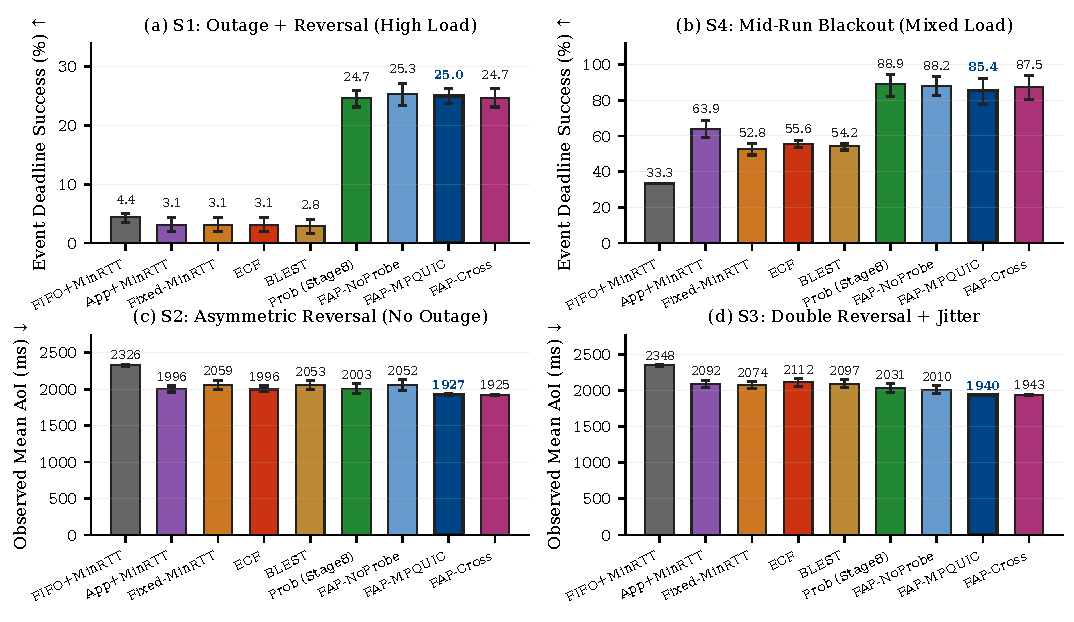
\includegraphics[width=\textwidth]{figures/fig02_stage10_main.pdf}
\caption{Held-out real \texttt{XQUIC} dual-path evaluation (576 connections, 16 seeds, 95\% seed-bootstrap CIs): (a)--(b) event deadline success on outage/blackout scenarios S1 and S4 (higher is better); (c)--(d) observed receiver mean state AoI on pure asymmetric and double reversals S2 and S3 (lower is better).}
\label{fig:main}
\end{figure*}

\begin{table*}[t]
\centering
\caption{Held-Out Real \texttt{XQUIC} Dual-Path Summary Across 4 Dynamic Scenarios (16 Seeds = 576 Connections)}
\label{tab:main}
\scriptsize
\setlength{\tabcolsep}{3.6pt}
\begin{tabular}{@{}llccccc@{}}
\toprule
Scenario & Policy Arm & EvSucc (\%) $\uparrow$ & AoI (ms) $\downarrow$ & GP (kbps) $\uparrow$ & Path-B (\%) & \texttt{FAP-MPQUIC} vs.\ Arm ($\Delta$Ev / $\Delta$AoI / $\Delta$GP) \\
\midrule
\multirow{7}{*}{S1: Outage+Rev}
& FIFO + MinRTT & 4.38 & 2644.2 & 93.8 & 94.7 & \textbf{+20.62\,pp}$^\dagger$ / \textbf{$-$743.6\,ms}$^\dagger$ / \textbf{+15.9\,k}$^\dagger$ \\
& App + MinRTT & 3.12 & 1993.1 & 87.4 & 94.4 & \textbf{+21.88\,pp}$^\dagger$ / $-$92.6\,ms / \textbf{+22.3\,k}$^\dagger$ \\
& Fixed-MinRTT & 3.12 & 2194.4 & 144.5 & 80.8 & \textbf{+21.88\,pp}$^\dagger$ / \textbf{$-$293.9\,ms}$^\dagger$ / $-$34.8\,k$^\dagger$ \\
& ECF~\cite{lim2017ecf} & 3.12 & 2195.2 & 144.0 & 80.8 & \textbf{+21.88\,pp}$^\dagger$ / \textbf{$-$294.6\,ms}$^\dagger$ / $-$34.4\,k$^\dagger$ \\
& BLEST~\cite{ferlin2016blest} & 2.81 & 2245.7 & 147.9 & 81.1 & \textbf{+22.19\,pp}$^\dagger$ / \textbf{$-$345.2\,ms}$^\dagger$ / $-$38.2\,k$^\dagger$ \\
& Prob-Only & 24.69 & 1878.1 & 109.9 & 86.8 & +0.31\,pp (n.s.) / +22.5\,ms (n.s.) / $-$0.2\,k \\
& \textbf{FAP-MPQUIC} & \textbf{25.00} & \textbf{1900.6} & \textbf{109.7} & \textbf{87.1} & Ref.\ (NoProbe: 25.31\%, 1875\,ms) \\
\midrule
\multirow{7}{*}{S2: Asym.\ Rev.}
& FIFO + MinRTT & 20.00 & 2326.4 & 109.8 & 59.8 & +0.62\,pp / \textbf{$-$399.3\,ms}$^\dagger$ / +7.5\,k \\
& App + MinRTT & 20.00 & 1996.4 & 111.0 & 60.0 & +0.62\,pp / \textbf{$-$69.4\,ms}$^\dagger$ / +6.3\,k \\
& Fixed-MinRTT & 20.00 & 2058.8 & 104.5 & 45.5 & +0.62\,pp / \textbf{$-$131.7\,ms}$^\dagger$ / +12.8\,k \\
& ECF~\cite{lim2017ecf} & 20.00 & 1995.9 & 112.9 & 49.7 & +0.62\,pp / \textbf{$-$68.9\,ms}$^\dagger$ / +4.4\,k \\
& BLEST~\cite{ferlin2016blest} & 20.00 & 2052.6 & 102.5 & 44.4 & +0.62\,pp / \textbf{$-$125.6\,ms}$^\dagger$ / +14.8\,k \\
& Prob-Only & 20.00 & 2003.3 & 113.6 & 78.2 & +0.62\,pp / $-$76.3\,ms ($p_{\text{raw}}{=}0.016$) / +3.7\,k \\
& \textbf{FAP-MPQUIC} & \textbf{20.62} & \textbf{1927.0} & \textbf{117.3} & \textbf{79.6} & Ref.\ (NoProbe: 2052.2\,ms; Cross: 1925.3) \\
\midrule
\multirow{8}{*}{S3: Double Rev.}
& FIFO + MinRTT & 20.00 & 2348.2 & 111.4 & 32.8 & +0.31\,pp / \textbf{$-$408.6\,ms}$^\dagger$ / +3.2\,k \\
& App + MinRTT & 20.00 & 2092.1 & 111.3 & 30.9 & +0.31\,pp / \textbf{$-$152.5\,ms}$^\dagger$ / +3.2\,k \\
& Fixed-MinRTT & 20.00 & 2074.2 & 101.2 & 24.0 & +0.31\,pp / \textbf{$-$134.5\,ms}$^\dagger$ / \textbf{+13.4\,k}$^\dagger$ \\
& ECF~\cite{lim2017ecf} & 20.00 & 2112.4 & 113.0 & 7.9 & +0.31\,pp / \textbf{$-$172.7\,ms}$^\dagger$ / +1.6\,k \\
& BLEST~\cite{ferlin2016blest} & 20.00 & 2096.7 & 103.9 & 25.0 & +0.31\,pp / \textbf{$-$157.1\,ms}$^\dagger$ / +10.7\,k \\
& Prob-Only & 20.62 & 2031.5 & 114.9 & 50.4 & $-$0.31\,pp / $-$91.9\,ms ($p_{\text{raw}}{=}0.015$) / $-$0.3\,k \\
& FAP-NoProbe & 20.31 & 2009.7 & 117.2 & 49.2 & +0.00\,pp / \textbf{$-$70.1\,ms}$^\dagger$ ($p_{\text{Holm}}{=}0.012$) / $-$2.6\,k \\
& \textbf{FAP-MPQUIC} & \textbf{20.31} & \textbf{1939.6} & \textbf{114.6} & \textbf{58.9} & Ref.\ (Cross: 20.00\%, 1942.9\,ms) \\
\midrule
\multirow{7}{*}{S4: Mid-Blackout}
& FIFO + MinRTT & 33.33 & 1786.4 & 78.6 & 76.1 & \textbf{+52.08\,pp}$^\dagger$ / \textbf{$-$871.7\,ms}$^\dagger$ / +1.2\,k \\
& App + MinRTT & 63.89 & 1222.3 & 70.1 & 70.8 & \textbf{+21.53\,pp}$^\dagger$ / \textbf{$-$307.7\,ms}$^\dagger$ / \textbf{+9.8\,k}$^\dagger$ \\
& Fixed-MinRTT & 52.78 & 1132.9 & 70.3 & 45.9 & \textbf{+32.64\,pp}$^\dagger$ / \textbf{$-$218.2\,ms}$^\dagger$ / \textbf{+9.5\,k}$^\dagger$ \\
& ECF~\cite{lim2017ecf} & 55.56 & 1118.0 & 71.0 & 46.1 & \textbf{+29.86\,pp}$^\dagger$ / \textbf{$-$203.4\,ms}$^\dagger$ / \textbf{+8.9\,k}$^\dagger$ \\
& BLEST~\cite{ferlin2016blest} & 54.17 & 1082.8 & 71.0 & 46.6 & \textbf{+31.25\,pp}$^\dagger$ / \textbf{$-$168.2\,ms}$^\dagger$ / \textbf{+8.9\,k}$^\dagger$ \\
& Prob-Only & 88.89 & 901.6 & 81.6 & 86.5 & $-$3.47\,pp (n.s.) / +13.0\,ms (n.s.) / $-$1.8\,k \\
& \textbf{FAP-MPQUIC} & \textbf{85.42} & \textbf{914.6} & \textbf{79.8} & \textbf{83.5} & Ref.\ (Cross: 87.50\%, 926.7\,ms) \\
\bottomrule
\multicolumn{7}{@{}l@{}}{\scriptsize $^\dagger$Global Holm-Bonferroni significant ($p_{\text{Holm}} < 0.05$, 20,000 sign-flip permutations, 16 seeds). $+\Delta$Ev/$+\Delta$GP and $-\Delta$AoI favor \texttt{FAP-MPQUIC}.}
\end{tabular}
\end{table*}

\subsection{Layer 1: Dominance of Loss- and Slack-Aware Binding Under Blackouts (S1 \& S4)}
Fig.~\ref{fig:main}, Fig.~\ref{fig:pareto}, Fig.~\ref{fig:effects}, and Table~\ref{tab:main} show that under sudden Path-A blackouts, loss- and slack-aware probability binding (\texttt{Prob-Only} and \texttt{FAP-MPQUIC}) overwhelmingly beats all five classical RTT-based schedulers:
\begin{itemize}
\item \textbf{S1 (High-Load Outage-Reversal):} \texttt{FAP-MPQUIC} raises event deadline success to \textbf{25.00\%} vs.\ 4.38\% (\texttt{FIFO+MinRTT}), 3.12\% (\texttt{App+MinRTT}, \texttt{Fixed-MinRTT}, \texttt{ECF}), and 2.81\% (\texttt{BLEST})---a \textbf{+20.62 to +22.19\,pp} jump (Cohen's $d_z \in [5.43, 6.66]$, all $p_{\text{Holm}}{\le}0.0025$) while slashing state AoI by \textbf{$-$293.9 to $-$743.6\,ms} vs.\ \texttt{Fixed-MinRTT}, \texttt{ECF}, \texttt{BLEST}, and \texttt{FIFO+MinRTT} ($p_{\text{Holm}}{\le}0.0031$). Notably, \texttt{Fixed-MinRTT}, \texttt{ECF}, and \texttt{BLEST} achieve higher raw goodput (144--148\,kbps) only by delivering late, expired event packets after Path~A recovers.
\item \textbf{S4 (Mid-Connection Path-A Blackout):} \texttt{FAP-MPQUIC} \textbf{strictly Pareto-dominates all four classical path schedulers across all three metrics simultaneously}: \textbf{+21.53 to +32.64\,pp} event deadline success ($p_{\text{Holm}}{\le}0.0230$; +52.08\,pp vs.\ \texttt{FIFO+MinRTT}), \textbf{$-$168.2 to $-$307.7\,ms} state AoI ($p_{\text{Holm}}{\le}0.0063$; $-$871.7\,ms vs.\ \texttt{FIFO+MinRTT}), and \textbf{+8.86 to +9.80\,kbps} useful goodput ($p_{\text{Holm}}{\le}0.0072$). As Fig.~\ref{fig:pareto}(b) confirms, \texttt{Fixed-MinRTT}, \texttt{ECF}, and \texttt{BLEST} stall at 45.9--46.6\% Path-B share, whereas \texttt{FAP-MPQUIC} shifts 83.5\% of traffic cleanly onto Path~B. Crucially, \texttt{FAP-MPQUIC} ties statistically with \texttt{Prob-Only} in both S1 and S4 (all $p_{\text{Holm}}{=}1.0$), verifying Proposition~\ref{prop:fap}(ii): health-gating suppresses probes on dead Path~A so probing incurs \emph{zero} blackout penalty.
\end{itemize}

\begin{figure*}[t]
\centering
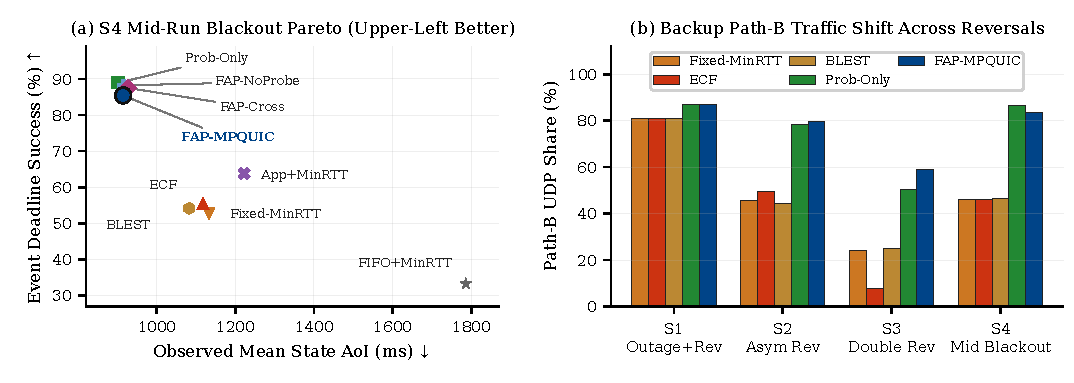
\includegraphics[width=\textwidth]{figures/fig03_pareto_and_path_shift.pdf}
\caption{Mechanistic separation across dynamic paths: (a) S4 mid-run blackout Pareto frontier showing \texttt{FAP-MPQUIC} and probability-based policies far in the optimal upper-left corner vs.\ \texttt{MinRTT}, \texttt{ECF}, and \texttt{BLEST}; (b) Path-B UDP utilization showing classical schedulers trapped on degraded Path~A in S2--S4 (especially \texttt{ECF} at 7.9\% in S3).}
\label{fig:pareto}
\end{figure*}

\begin{figure*}[t]
\centering
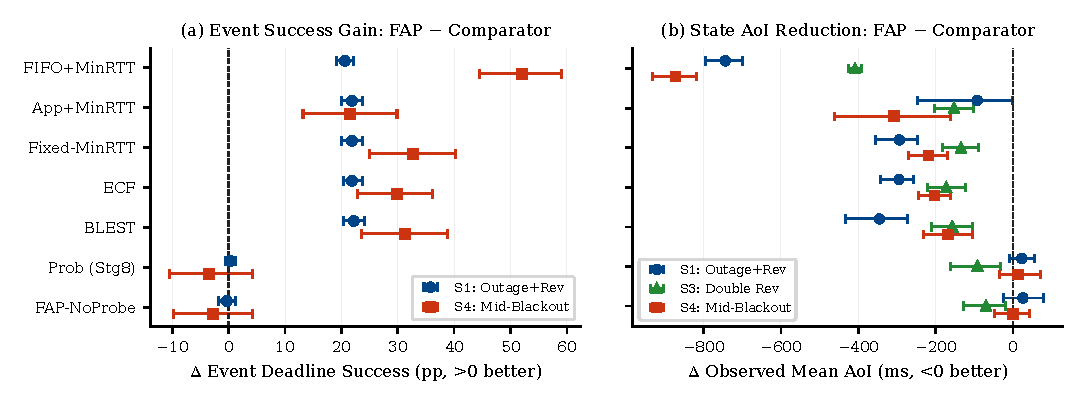
\includegraphics[width=\textwidth]{figures/fig04_paired_effects.pdf}
\caption{Paired 16-seed bootstrap 95\% confidence intervals (\texttt{FAP-MPQUIC} minus comparator): (a) event deadline success gains on S1 and S4; (b) state AoI reductions on S1, S3, and S4, including the Holm-significant $-$70.1\,ms AoI reduction of health-gated probing over \texttt{FAP-NoProbe} in S3.}
\label{fig:effects}
\end{figure*}

\subsection{Layer 2: Breaking the Stale-RTT Trap Under Non-Blackout Reversals (S2 \& S3)}
Under non-blackout asymmetric (S2) and bidirectional (S3) reversals, sudden loss does not automatically expel traffic from Path~A. Consequently, classical schedulers remain heavily pinned to degraded Path~A (\texttt{ECF} uses only 7.9\% Path~B in S3; \texttt{Fixed-MinRTT} and \texttt{BLEST} 24--25\%), \emph{and} both \texttt{Prob-Only} and \texttt{FAP-NoProbe} remain exposed to stale cached RTTs on the idle alternate path. Health-gated probing directly resolves this second layer, delivering the \textbf{lowest observed AoI of all 9 policies} in both S2 and S3:
\begin{itemize}
\item In \textbf{S2}, \texttt{FAP-MPQUIC} achieves \textbf{1,927.0\,ms} AoI (Holm-significant vs.\ all five classical baselines: $-$68.9 to $-$399.3\,ms, $p_{\text{Holm}}{\le}0.0034$) and the highest goodput among strict policies (117.3\,kbps), cutting AoI by $-$76.3\,ms over \texttt{Prob-Only} ($p_{\text{raw}}{=}0.0162$) and $-$125.2\,ms over \texttt{FAP-NoProbe} ($p_{\text{raw}}{=}0.0126$).
\item In \textbf{S3}, \texttt{FAP-MPQUIC} achieves \textbf{1,939.6\,ms} AoI (Holm-significant vs.\ all five classical baselines: $-$134.5 to $-$408.6\,ms, $p_{\text{Holm}}{\le}0.0031$) and \textbf{Holm-significantly beats its own no-probe ablation \texttt{FAP-NoProbe} by $-$70.06\,ms} (95\% CI $[-128.0, -20.4]$\,ms, $p_{\text{Holm}}{=}0.0123$; $-$91.9\,ms vs.\ \texttt{Prob-Only}, $p_{\text{raw}}{=}0.015$), directly isolating the causal value of health-gated stale-path probing under bidirectional link reversals.
\end{itemize}

\subsection{Mechanism Analysis: Cross-Path Failover and Offline Calibration}
Two targeted supplementary mechanism evaluations (Fig.~\ref{fig:repair}) clarify failover and probability calibration trade-offs:
\begin{enumerate}
\item \textbf{Strict Affinity vs.\ Cross-Path Repair:} Across the general dual-path matrix (S1--S4), \texttt{FAP-MPQUIC} (strict) and \texttt{FAP-Cross} perform nearly identically (within 0.3--2.1\,pp and 2--12\,ms, all $p_{\text{Holm}}{=}1.0$). Yet under directed single-stream outages (20 independent seeds, Fig.~\ref{fig:repair}(a)), cross-path repair slashes mean probe completion from \textbf{1,544\,ms to 253\,ms} ($-$83.6\%, 95\% CI $[-1314, -1267]$\,ms) and cuts duplicate stream-offset UDP bytes from 24.1\,KB to 15.1\,KB.
\item \textbf{Offline Probability Calibration Boundary:} Across 1,031 held-out randomized-path delivery records (Fig.~\ref{fig:repair}(b)), offline Platt calibration reduces effective-budget Brier error from 0.0413 to \textbf{0.0355} (0.260 to 0.218 on 0--100\,ms short budgets), though short-budget calibrated gains over \texttt{Slack-only} remain modest under sudden distribution shift~\cite{ovadia2019uncertainty}.
\end{enumerate}

\begin{figure*}[t]
\centering
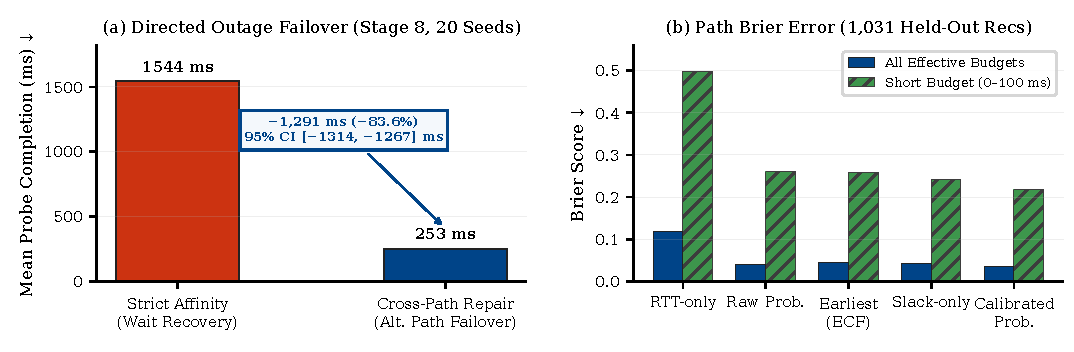
\includegraphics[width=\textwidth]{figures/fig05_repair_and_calibration.pdf}
\caption{Supplementary mechanism analyses: (a) directed single-stream outage failover across 20 seeds (cross-path repair cuts completion latency by $-$83.6\%); (b) held-out path-completion Brier score across 1,031 randomized-path test records.}
\label{fig:repair}
\end{figure*}

\section{Discussion and Limitations}
Our 1,596+ audited real-\texttt{XQUIC} connections offer two clear engineering principles for IoT gateway designers:
\begin{itemize}
\item \textbf{Layer 1 --- Loss- and Variance-Aware Binding Unlocks Outage Resilience:} Replacing pure-RTT schedulers (\texttt{MinRTT}/\texttt{ECF}/\texttt{BLEST}) with loss- and slack-aware probability binding unlocks +20--32\,pp event delivery under outages because pure RTT schedulers remain blind to sudden blackouts on previously fast links.
\item \textbf{Layer 2 --- Health Gating Makes Freshness Probing Safe Across Reversals and Blackouts:} Probing stale backup paths with replaceable state streams refreshes transport SRTTs in one QUIC RTT ($\approx$10--20\,ms vs.\ 950\,ms for app-ACK adaptation), lowering AoI by $-$70 to $-$125\,ms under reversals, while the $f_j{=}m_j{=}\text{pto}_j{=}0$ gate preserves full blackout resilience with zero credit waste.
\end{itemize}

\paragraph{Explicit Scope Limitations}
Three boundaries warrant future work. First, while both endpoints run unmodified \texttt{XQUIC}/\texttt{BoringSSL} over real Linux UDP sockets and \texttt{tc-netem}, both namespaces share one physical host rather than multi-hop physical Wi-Fi + cellular radios with real RF interference. Second, our connection concurrency is configured to $C{=}4$ unidirectional streams to represent resource-constrained IoT gateway budgets and expose bad-path credit blocking; higher \texttt{MAX\_STREAMS} credits would reduce queueing contention on high-mixed bursts. Third, our offline calibration analysis remains decoupled from online selection; integrating online shift-robust conformal calibration is a promising next step.

\section{Conclusion}
We presented \texttt{FAP-MPQUIC}, a lightweight, zero-control-overhead multipath scheduler built directly on production C \texttt{XQUIC} for mixed-traffic IoT gateways. By combining overwrite-freshness application scheduling, CWND-blocking-aware timely delivery estimation, and health-gated stale-path freshness probing with proved discovery and zero-blackout-waste bounds, \texttt{FAP-MPQUIC} achieves Holm-significant gains across 576 held-out real \texttt{XQUIC} connections---boosting event deadline delivery by +20.6 to +52.1\,pp over \texttt{MinRTT}, \texttt{ECF}, and \texttt{BLEST}, strictly Pareto-dominating all four classical path schedulers under mid-connection blackouts, and cutting state AoI by $-$70.1\,ms over its no-probe ablation under bidirectional reversals while preserving zero blackout credit waste.

\clearpage
\bibliographystyle{IEEEtran}
\bibliography{references}

\end{document}
